
A continuaci\'on mostramos varios ejemplos de derivaciones v\'alidas:

  \begin{itemize}

	\item{  Ejemplo 1: Html Empty.
		\begin{verbatim}
			<html>
			</html> 
		\end{verbatim}
	}


\begin{center}
	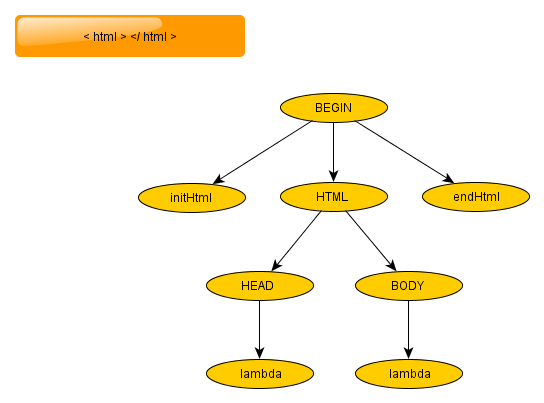
\includegraphics[scale=0.5]{Imagenes/1_html_empty.png}\\
\end{center}

	\item{  Ejemplo 2: Empty head body with text.
		\begin{verbatim}
			<html> 
			   <body> 
			      <br> Body text <br> 
			   </body> 
			</html> 
		\end{verbatim}
	}

\begin{center}
	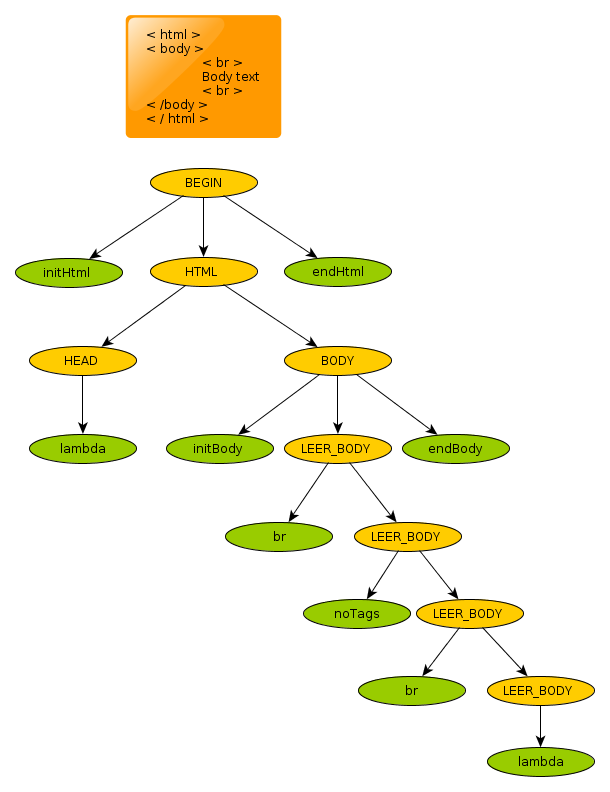
\includegraphics[scale=0.44]{Imagenes/2_empty_head_body_with_text.png}\\
\end{center}

\newpage

	\item{  Ejemplo 3: Tp example.
		\begin{verbatim}
			<html>
			   <head>
			      <title>Esto es un titulo</title>
			      <script> print("Hola mundo")</script>
			   </head>
			   <body> Esto es 
			      <p>
			         una
			         <h1>
			            prueba
			         </h1>
			      </p> 
			      <br> 
			   </body>
			</html> 
		\end{verbatim}
	}

\begin{center}
	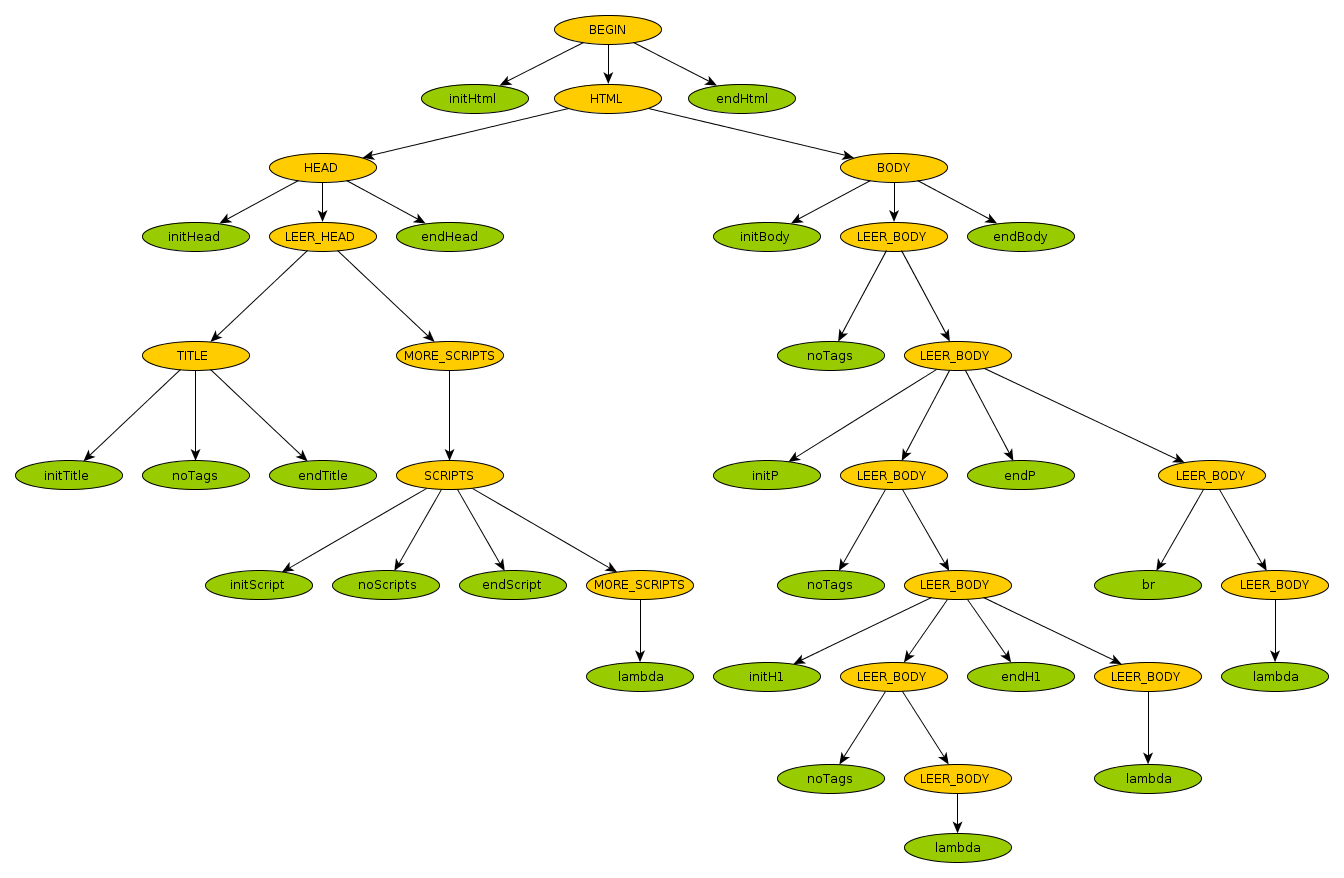
\includegraphics[scale=0.33]{Imagenes/3_tp_example.png}\\
\end{center}

\newpage

	\item{  Ejemplo 4: Huge Body.
		\begin{verbatim}
			<html>
			   <head>
			      <title> Something's Gone Terribly Wrong </title>
			      <script> </script>
			      <script> bN_cfg = {p: {"dL_ch":"us.hpmguncat",
			               "dL_dpt":"error","cobrand":"HuffPost"}};
			      </script>
			   </head>
			   <body>
			      <div> </div>
			      <div>
			         <h1> Oh, Noes! A 404! </h1>
			         <div> 
			            <div> </div> 
			            <p> or </p> 
			         </div> 
			      </div>
			   </body> 
			</html>
		\end{verbatim}

	}

\begin{center}
	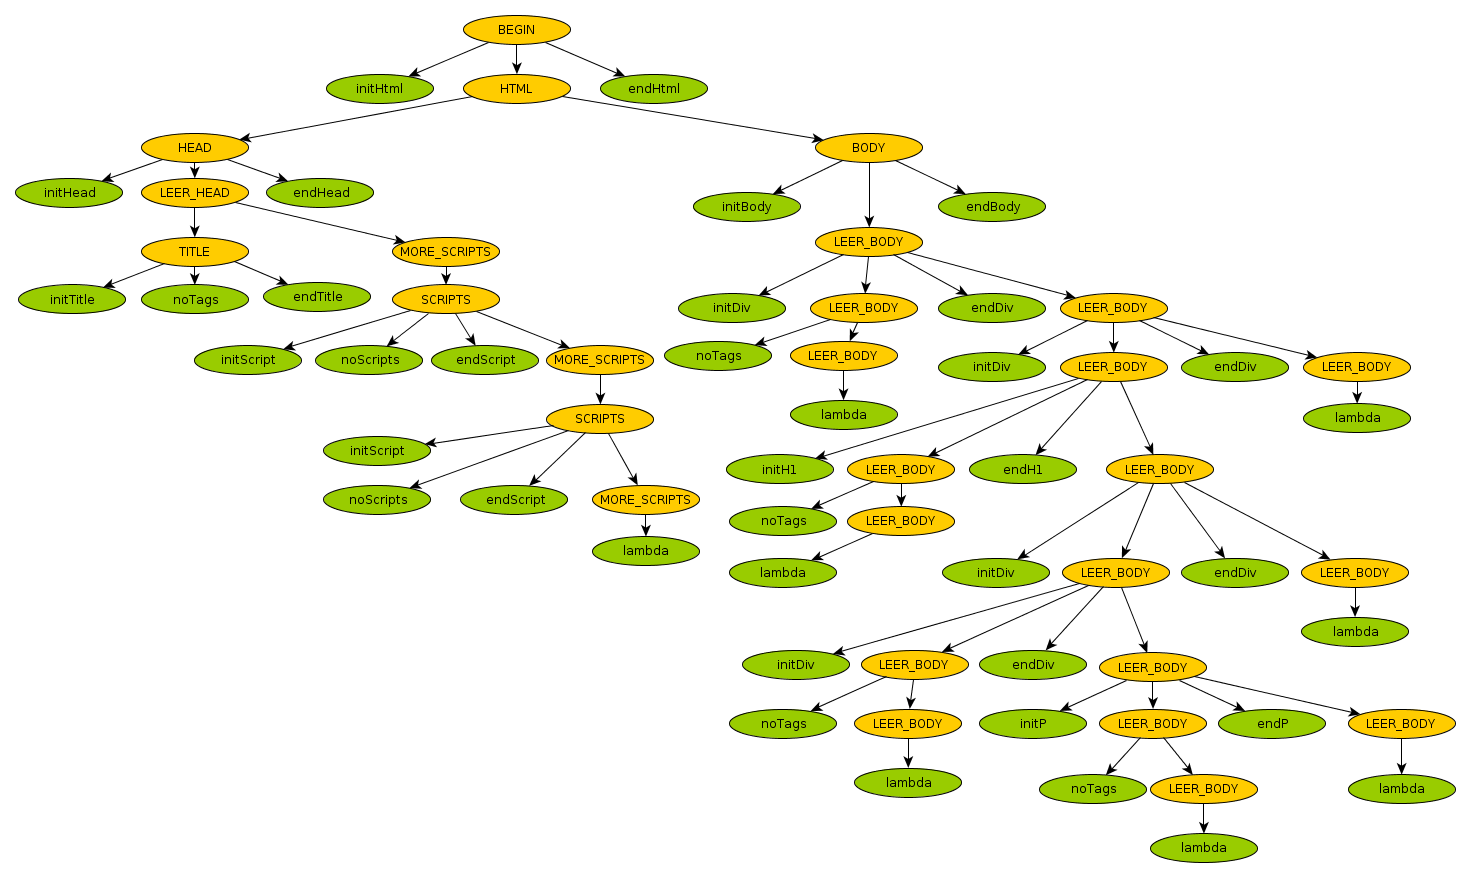
\includegraphics[scale=0.30]{Imagenes/4_huge_body.png}\\
\end{center}

\newpage

	\item{  Ejemplo 5: Just title empty body.
		\begin{verbatim}
			<html> 
			   <head>
			      <title> reddit </title> 
			   </head>
			   <body> 
			      Posts 
			   </body>
			</html>
		\end{verbatim}

	}

\begin{center}
	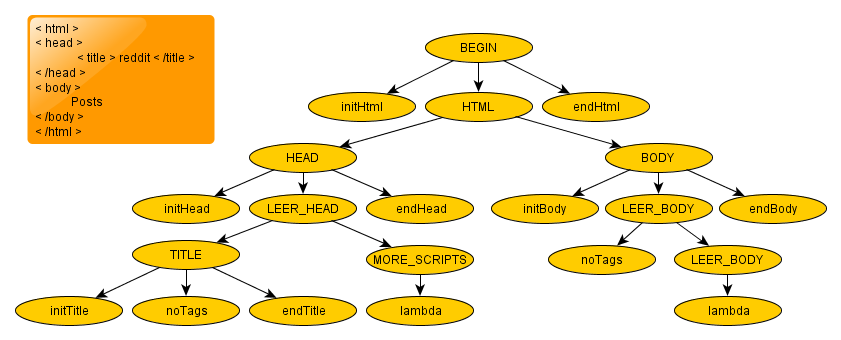
\includegraphics[scale=0.5]{Imagenes/5_just_title_empty_body.png}\\
\end{center}

\newpage

	\item{  Ejemplo 6: Several scripts middle title no body.
		\begin{verbatim}
			<html>
			   <head> 
			      <script> $(".container").append("<h1> Header </h1>"); </script> 
			      <script> Tenemos varios scripts </script > 
			      <title> Esto es un titulo </title>
			      <script> print("Title en medio (Y)") </script> 
			   </head> 
			</html> 
		\end{verbatim}

	}

\begin{center}
	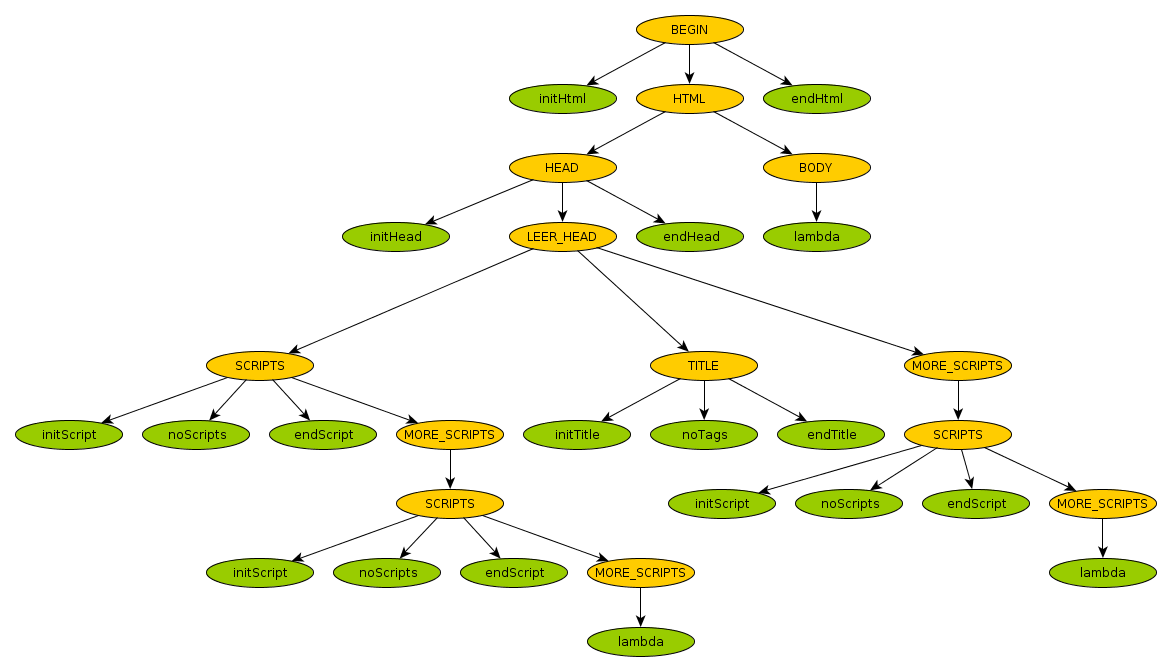
\includegraphics[scale=0.40]{Imagenes/6_several_scripts_middle_title_no_body.png}\\
\end{center}

\newpage

	\item{  Ejemplo 7: Just scripts nested tags and text.
		\begin{verbatim}
			<html>
			   <head> 
			      <script> <div> Solo scripts </div> </script> 
			      <script> <div> Sin title </div> </script>
			   </head>
			   <body> 
			      <br> 
			      <div>
			         <p> Tags anidados </p> 
			         aca 
			      </div> 
			      Y texto suelto
			   </body>
			</html>
		\end{verbatim}

	}

\begin{center}
	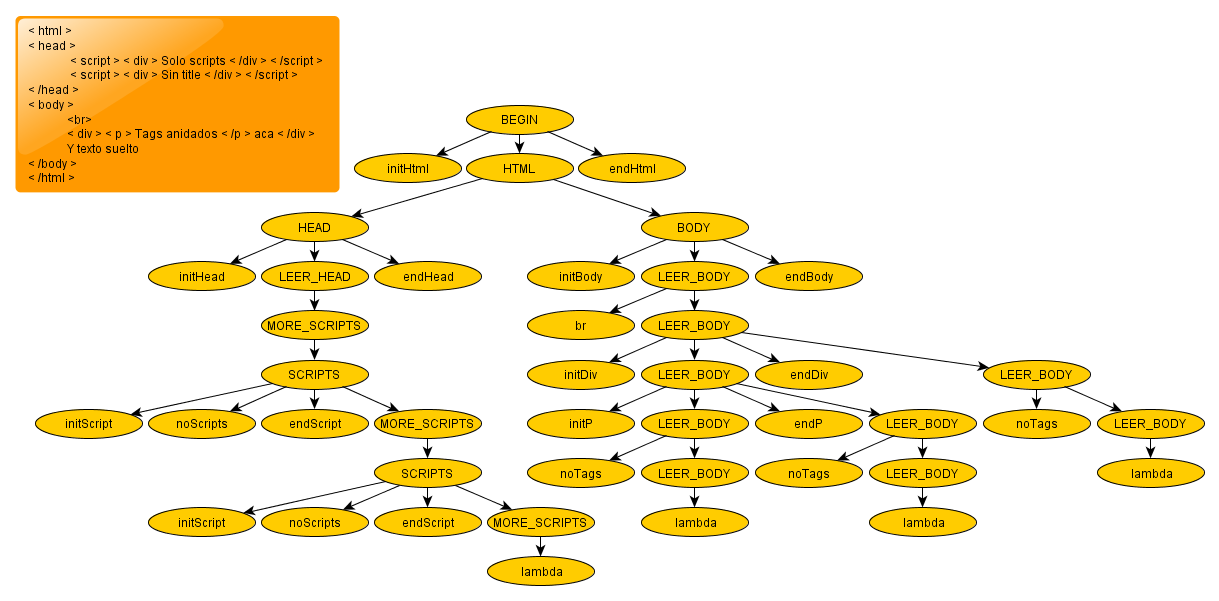
\includegraphics[scale=0.37]{Imagenes/7_just_scripts_nested_tags_and_text.png}\\
\end{center}

  \end{itemize}
